\documentclass[11pt]{article}
\usepackage[T1]{fontenc}
\usepackage[utf8]{inputenc}
\usepackage{lmodern,amsmath,booktabs,graphicx,longtable,float}
\usepackage[margin=1in]{geometry}
\usepackage[round,authoryear]{natbib}
\usepackage[hidelinks]{hyperref}
\bibliographystyle{apalike}
\newcommand{\nSnapFar}{1,020}
\newcommand{\ratioMin}{32}
\newcommand{\ratioMax}{59}
\newcommand{\rhoRatioPdH}{-0.40}
\newcommand{\rhoDeadEndRatio}{-0.65}
\newcommand{\rhoCircuityRatio}{-0.63}
\newcommand{\rhoMeshRatio}{0.69}
\newcommand{\rhoFragRatio}{0.09}
\newcommand{\rhoDeadEndPdH}{0.40}
\newcommand{\rhoFragPdH}{-0.12}
\newcommand{\meanPdHPopmatch}{-1.6}
\newcommand{\meanDHPopmatch}{-0.0003}
\newcommand{\sharePositivePopmatch}{20.9}
\newcommand{\spearmanPopmatch}{0.999}
\newcommand{\envPopRatio}{50}
\newcommand{\medianPopmatchB}{1,330}
\newcommand{\maxDH}{0.026}
\newcommand{\minPdH}{0.8}
\newcommand{\nCities}{91}
\newcommand{\nFailed}{0}
\newcommand{\nTractsUrban}{151,992}
\newcommand{\sharePopUrban}{98.9}
\newcommand{\meanHeuc}{0.022}
\newcommand{\meanHnet}{0.028}
\newcommand{\meanDH}{0.005}
\newcommand{\meanPdH}{29.8}
\newcommand{\maxPdH}{109.0}
\newcommand{\sharePositive}{100.0}
\newcommand{\pearsonMain}{0.980}
\newcommand{\spearmanMain}{0.984}
\newcommand{\nRankChangeTop}{11}


\title{Segregated by Design in Brazil? Street-Network Topology and the Measurement of Racial Segregation}
\author{Renan Xavier Cortes}
\date{\today}

\begin{document}
\maketitle

\begin{abstract}
Spatial segregation indices usually define each resident's local environment with straight-line distance,
although people move along streets. Following \citet{knaap2024segregated}, we compare racial segregation measured
with Euclidean and with pedestrian network distance for the \nCities{} Brazilian municipalities with at least
300,000 inhabitants, using 2022 Census colour-or-race counts for \nTractsUrban{} urban tracts and OpenStreetMap
walking networks. The two local environments share an identical 2-km kernel and differ only in the distance
metric. With network distance, the multigroup spatial information theory index is higher in every city, by
\meanPdH\% on average, and the ranking of the most segregated cities changes, with hilly and island cities such
as Florian\'opolis and Vit\'oria climbing. However, 2-km walking environments contain only about \envPopRatio\% of
the population of 2-km circles. When Euclidean environments are shrunk to hold the same population, the gap
vanishes (mean difference \meanPdHPopmatch\%). Across cities the gap and the share of reachable population are
associated with dead-end streets, circuity and meshedness, but not with a metric analogue of the space-syntax
fragmentation that characterises Brazilian street grids. Street networks thus shape measured segregation mainly
by setting the effective scale of neighbourhoods, which argues for population-matched comparisons and points to
local street permeability as a planning lever. All analyses use the open-source PySAL \texttt{segregation}
package and are fully reproducible.
\end{abstract}
\noindent\textbf{Keywords:} residential segregation; street networks; spatial weights; urban morphology;
OpenStreetMap; Brazil; PySAL


\section{Introduction}\label{sec:intro}

Straight-line distance is the default abstraction of applied spatial analysis. It is a useful simplification,
but people do not move across a featureless plane: they walk along streets, around blocks, over bridges and up
stairways, and the configuration of that network conditions whom they can easily meet. In segregation research
the abstraction enters through the definition of the ``local environment'' that spatial indices compare with the
city as a whole \citep{reardon2004measures}. Most applications define that environment with Euclidean distance.
\citet{knaap2024segregated} showed, for every metropolitan area in the United States, that replacing Euclidean
distance with walking distance along the street network raises the spatial information theory index in almost
every metro, by about a fifth on average, and reshuffles the ranking of the most segregated places. They also
showed that the size of the gap is associated with the topology of the street network.

This paper asks whether the same holds in Brazil, where there are strong reasons to expect the street network to
matter even more. Brazilian cities combine colonial cores, modernist plans, sprawling peripheral \emph{loteamentos},
self-built favelas on steep hillsides and, since the 1990s, gated condominiums (\emph{condom\'inios fechados}) that
interrupt the public street grid \citep{coy2006gated}. In the most comprehensive configurational comparison to
date, \citet{medeiros2013urbis} found that the street networks of the 27 Brazilian state capitals are among the
most fragmented of 164 cities worldwide: a ``patchwork'' of locally coherent pieces that are poorly articulated
with one another. If segregation is, in part, a restriction on the possibility of interaction
\citep{netto2015segregated}, then a patchwork city should look more segregated when the local environment is
measured along the network than when it is measured as the crow flies.

We compute racial segregation for the \nCities{} Brazilian municipalities with at least 300,000 inhabitants,
using the 2022 Census colour-or-race counts for urban census tracts and pedestrian networks from OpenStreetMap.
For each city we build two local environments that differ \emph{only} in the distance metric: the same 2-km
triangular kernel is applied to Euclidean and to network distances. We ask two questions. First, how different
are segregation levels and rankings under the two metrics (RQ1)? Second, which properties of the street network
are associated with the gap (RQ2)? To RQ2 we add a Brazil-specific predictor, a metric analogue of the
space-syntax \emph{synergy} measure that underlies Medeiros's diagnosis of fragmentation. Because network
environments contain fewer people than Euclidean environments of the same radius, part of any gap could be a
scale effect rather than a barrier effect \citep{saporito2026reconsidering}; we therefore also report a
population-matched comparison in which each tract's Euclidean environment is shrunk until it holds as many
people as its network environment.

The paper makes three contributions: the first nationwide Euclidean-versus-network comparison of segregation for
a country of the Global South; a test of whether configurational fragmentation, a long-standing theme of
Brazilian urban morphology, helps explain the gap; and a fully reproducible workflow built on the open-source
PySAL \texttt{segregation} package \citep{cortes2026segregation,cortes2020open,rey2021comparative,rey2022pysal}.
Consistent with \citet{knaap2024segregated}, we treat the comparison descriptively; a formal inferential test of
the gap is left for future work.

\section{Background}\label{sec:background}

\subsection{Measuring segregation in space}

Spatial segregation indices replace the question ``who lives in the same tract?'' with ``who lives nearby?''.
\citet{white1983measurement} introduced distance decay into the measurement of segregation, and
\citet{wong1993spatial} showed that indices based on the adjacency of areal units depend on unit size and shape.
\citet{reardon2004measures} provided a general framework in which any theoretically motivated proximity function
defines each person's local environment; among the resulting measures, the spatial information theory index $H$
has the most desirable properties. \citet{reardon2008geographic} used the bandwidth of the proximity function to
describe the geographic scale of segregation. In Brazil, \citet{feitosa2007global} developed kernel-based global
and local spatial indices and applied them to S\~ao Jos\'e dos Campos. In all of these, proximity is almost always
Euclidean.

\subsection{Street networks and social interaction}

A second literature argues that street networks structure the opportunities for contact.
\citet{grannis1998importance} showed that residential (``trivial'') streets bound neighbourhood networks, and
\citet{grannis2005tcommunities} that pedestrian-connected ``T-communities'' predict racial composition in three US
cities. \citet{roberto2018spatial} incorporated road connectivity into segregation measurement and found higher
segregation in Pittsburgh under network distance. \citet{knaap2024segregated} scaled this comparison to all US
metros and related the gap to network topology measured with OSMnx \citep{boeing2017osmnx} and momepy
\citep{fleischmann2019momepy}: circuity widens the gap, intersection density narrows it, and cyclomatic
complexity (redundancy) dampens the effect of circuity. Global comparisons show that street-network form varies
far more outside North America: grids are the exception, and circuity and orientation entropy are higher
\citep{boeing2019urban,boeing2022street}. Recently, \citet{saporito2026reconsidering} cautioned that network-based
environments of a given radius contain fewer people, so that part of the network--Euclidean difference may reflect
the population size of local environments rather than barriers to movement.

\subsection{The configuration of Brazilian street networks}

Brazilian research on urban form has long emphasised configuration. Drawing on space syntax,
\citet{holanda2002espaco} interpreted the plan of Bras\'ilia as a ``space of exception'' whose dispersed,
hierarchical layout separates social groups. \citet{medeiros2013urbis} compared axial maps of 164 cities, including
all 27 Brazilian capitals, and concluded that Brazilian cities are exceptionally fragmented: patchworks of
internally coherent pieces whose local and global structures are poorly articulated (low \emph{synergy}), a
labyrinthine configuration that hampers movement between parts of the city. \citet{netto2015segregated} reframed
segregation as a restriction on interaction produced jointly by residential location, the street network and
mobility, with evidence from a Brazilian city. Two recent studies bring the street grid directly into segregation
measurement: \citet{saboya2025chasm} propose CHASM, an exposure measure computed on street segments, and
\citet{goncalves2024uncovering} use a network-based potential-accessibility index to reveal racial and income
segregation patterns in Pelotas. At the scale of informal settlements, \citet{carvalho2023segregation} show that
favelas are themselves internally segregated. Using OSM, \citet{spadon2018topological} characterised the street
networks of the 645 municipalities of S\~ao Paulo state by topological features. Finally, the spread of gated
condominiums has privatised parts of the street network and fragmented the urban fabric \citep{coy2006gated}.
Together these works motivate three expectations: (H1) segregation is higher under network than under Euclidean
distance; (H2) the gap is larger where circuity, dead-end streets and configurational fragmentation are higher;
and (H3) the gap is smaller where intersection density and meshedness are higher.

\subsection{Race, space and access in Brazilian cities}

Racial residential segregation in Brazil is moderate by US standards but real and entangled with class
\citep{telles2004race}; a nationwide analysis of 2010 census tracts found it highest in the South and Southeast
\citep{sousafilho2023segregacao}. The consequences of location are mediated by the transport network. The IPEA
\emph{Acesso a Oportunidades} project shows that white and high-income residents of the 20 largest Brazilian
cities reach more jobs, schools and health services than black and low-income residents by every transport mode
\citep{pereira2019desigualdades,tomasiello2024racial}, and that transport policy can widen these gaps
\citep{pereira2019distributional}. \citet{bittencourt2021cumulative} show that accessibility and segregation
reinforce each other in four metropolises, and \citet{boisjoly2020accessibility} document large accessibility
differences across four cities. This literature measures travel along networks
\citep{pereira2021r5r} but takes residential segregation as given; our study brings the network into the
measurement of segregation itself.

\section{Data and methods}\label{sec:methods}

\subsection{Cities, tracts and population groups}

The study covers the \nCities{} municipalities with a 2022 Census population of at least 300,000, a set that
includes all 27 state capitals. The spatial units are 2022 census tracts (\emph{setores censit\'arios}). We keep
tracts classified as urban (\texttt{SITUACAO} = \emph{Urbana}) with at least one resident, \nTractsUrban{} tracts
holding \sharePopUrban\% of the population of the \nCities{} municipalities. We restrict the analysis to urban
tracts because several municipalities (e.g.\ Porto Velho or Manaus) contain very large rural tracts whose
centroids lie kilometres from any street, which would inflate network distances for reasons unrelated to urban
design. Population counts come from the Census tract aggregates for colour or race: \emph{branca}, \emph{preta},
\emph{amarela}, \emph{parda} and \emph{ind\'igena}. Cells suppressed for confidentiality are set to zero.

\subsection{Street networks}

For each municipality we download the OpenStreetMap pedestrian network (all ways usable on foot, including
footpaths and stairways) with OSMnx \citep{boeing2017osmnx} for the union of its urban tracts buffered by 2~km, so
that walking paths may leave the urban footprint. Graphs are simplified, projected to the SIRGAS~2000 UTM zone of
the city, made undirected, and reduced to their largest connected component. Each tract is represented by a
point guaranteed to lie inside the polygon and snapped to the nearest network node; the snap distance is kept and
added to network distances.

\subsection{Local environments and the segregation index}

Let $d_{ij}$ be the distance between tracts $i$ and $j$. We use two distances: Euclidean $d^{E}_{ij}$, and network
$d^{N}_{ij} = s_i + \ell(n_i, n_j) + s_j$, where $n_i$ is the node nearest to tract $i$, $s_i$ the snap distance and
$\ell$ the shortest-path length. Because the snapped path is itself a path between the two points,
$d^{N}_{ij} \geq d^{E}_{ij}$. Both distances enter the same triangular kernel,
\begin{equation}
  w_{ij} = \begin{cases} 1 - d_{ij}/b & \text{if } d_{ij} \le b,\\ 0 & \text{otherwise,}\end{cases}
  \qquad w_{ii} = 1,
  \label{eq:kernel}
\end{equation}
with bandwidth $b = 2{,}000$~m, as in \citet{knaap2024segregated}. The local environment of tract $i$ is the
spatially weighted population $\tilde{\tau}_{im} = \sum_j w_{ij}\tau_{jm}$ of each group $m$, and
$\tilde{\pi}_{im} = \tilde{\tau}_{im} / \sum_m \tilde{\tau}_{im}$. The entropy of each local environment is
$\tilde{E}_i = -\sum_m \tilde{\pi}_{im}\ln\tilde{\pi}_{im}$, and the spatial information theory index is
\begin{equation}
  H = 1 - \frac{1}{T E}\sum_i \tilde{t}_i \tilde{E}_i ,
  \label{eq:H}
\end{equation}
where $\tilde t_i$ is the local population, $T$ the total population and $E$ the city-wide entropy
\citep{reardon2004measures}. $H$ equals 0 when every local environment has the city's composition and 1 when every
local environment contains a single group. We compute $H$ over the five colour-or-race groups (a group absent from
a city contributes zero). As secondary measures we compute the spatial versions of dissimilarity, isolation and
entropy for the \emph{preta}+\emph{parda} population. All indices are computed with the PySAL \texttt{segregation}
package \citep{cortes2026segregation,cortes2020open}. We build the weighted local environments with a sparse
matrix product identical to the one the package applies to a \texttt{libpysal} weights object, which a unit test
verifies to machine precision, and then call the package's estimators. For each city we record
$H^{E}$, $H^{N}$, the gap $\Delta H = H^{N} - H^{E}$ and the relative gap $\%\Delta H = 100\,\Delta H / H^{E}$.

\paragraph{Population-matched environments.} Because $d^{N}_{ij} \ge d^{E}_{ij}$, a network environment of radius
$b$ always contains fewer (weighted) people than a Euclidean one, and smaller environments are, other things equal,
less diverse. Following the concern raised by \citet{saporito2026reconsidering}, we also compare $H^{N}$ with a
Euclidean index computed from \emph{population-matched} environments: for each tract we find, by bisection, the
Euclidean radius $b_i \le 2{,}000$~m at which the kernel-weighted population of its Euclidean environment equals
that of its 2-km network environment, and recompute $H$ with these tract-specific radii. Any remaining gap cannot
be attributed to the number of people in local environments.

\subsection{Network topology and configurational fragmentation}

Topology is measured on all network nodes lying inside the urban footprint (the union of populated urban
tracts). We keep every piece rather than only the largest component, because planned cities such as Palmas
consist of superblocks that connect through streets outside the footprint. Table~\ref{tab:topodef} lists the
measures, which follow \citet{knaap2024segregated}. Densities are expressed per km$^2$ of footprint.

\begin{table}[htbp]
\centering\small
\caption{Street-network topology measures ($v$ nodes, $e$ edges, $p$ connected components).}\label{tab:topodef}
\begin{tabular}{p{4.2cm}p{9.3cm}}
\toprule
Measure & Definition \\
\midrule
Intersection density & nodes with degree $\ge 3$ per km$^2$ \\
Street density & km of street per km$^2$ \\
Mean street length & mean edge length (m) \\
Streets per node & mean node degree (parallel edges counted) \\
Circuity & $\sum$ edge length $/ \sum$ straight-line length between edge endpoints \\
Dead-end, 3-way, 4-way shares & share of nodes with degree 1, 3 and 4 \\
Cyclomatic number & $e - v + p$ (independent loops; network redundancy) \\
Meshedness & $(e - v + p)/(2v - 5)$ (share of the maximum possible number of loops) \\
Gamma & $e / 3(v - 2)$ \\
Fragmentation $F$ & $1 - \operatorname{corr}(\ln L_i, G_i)$, see text \\
\bottomrule
\end{tabular}
\end{table}

\paragraph{Configurational fragmentation.} Space syntax diagnoses a ``patchwork'' city by the weak correlation
(low \emph{synergy}) between the local and global integration of its street segments \citep{medeiros2013urbis}.
Axial maps are not available for \nCities{} cities, so we compute a metric analogue on the OSM graph. For a node
$i$, local reach $L_i$ is the total street length whose two endpoints lie within 800~m of network distance from
$i$. Global closeness $G_i$ is the reciprocal of the mean network distance from $i$ to 500 randomly drawn urban
nodes. Synergy is the Pearson correlation between $\ln L_i$ and $G_i$ over 2,000 randomly drawn urban nodes,
and fragmentation is $F = 1 - \text{synergy}$. Routing uses the full buffered network. High $F$ means that
locally well-connected places are not necessarily well connected to the city as a whole. We stress that $F$
approximates the space-syntax measure with metric distances rather than replicating it.

\subsection{Analytical strategy}

For RQ1 we describe the distributions of $H^{E}$, $H^{N}$, $\Delta H$ and $\%\Delta H$, their Pearson and Spearman
correlations and the change in the ranking of the most segregated cities, and we repeat the comparison with
bandwidths of 1 and 3~km, an exponential kernel ($w = e^{-3d/b}$), the secondary indices and the
population-matched environments. For RQ2 we estimate, across cities,
\begin{equation}
  y_c = \alpha + \mathbf{x}_c'\boldsymbol\beta + \varepsilon_c ,
\end{equation}
with $y_c \in \{\Delta H, \%\Delta H\}$. $\mathbf{x}_c$ contains log intersection density, circuity, meshedness,
log cyclomatic number, dead-end share, log population density and $H^{E}$, plus the cyclomatic$\times$circuity
interaction of \citet{knaap2024segregated}. We then add $F$ and compare the fit. Normally distributed regressors
are standardised and skewed ones logged. Standard errors are heteroskedasticity-robust (HC3). With
$N = \nCities{}$ the models are descriptive associations, not causal estimates.

\section{Results}\label{sec:results}

\subsection{How much does the distance metric matter?}

Figure~\ref{fig:vignettes} illustrates the difference between the two local environments for three contrasting
fabrics. In Goi\^ania's planned grid the area reachable within 2~km on foot fills much of the 2-km circle. In the
hillside neighbourhoods of Rio de Janeiro and in Salvador, whose street network is organised around ridges and
valleys, it covers a small, irregular part of it.

\begin{figure}[htbp]
\centering
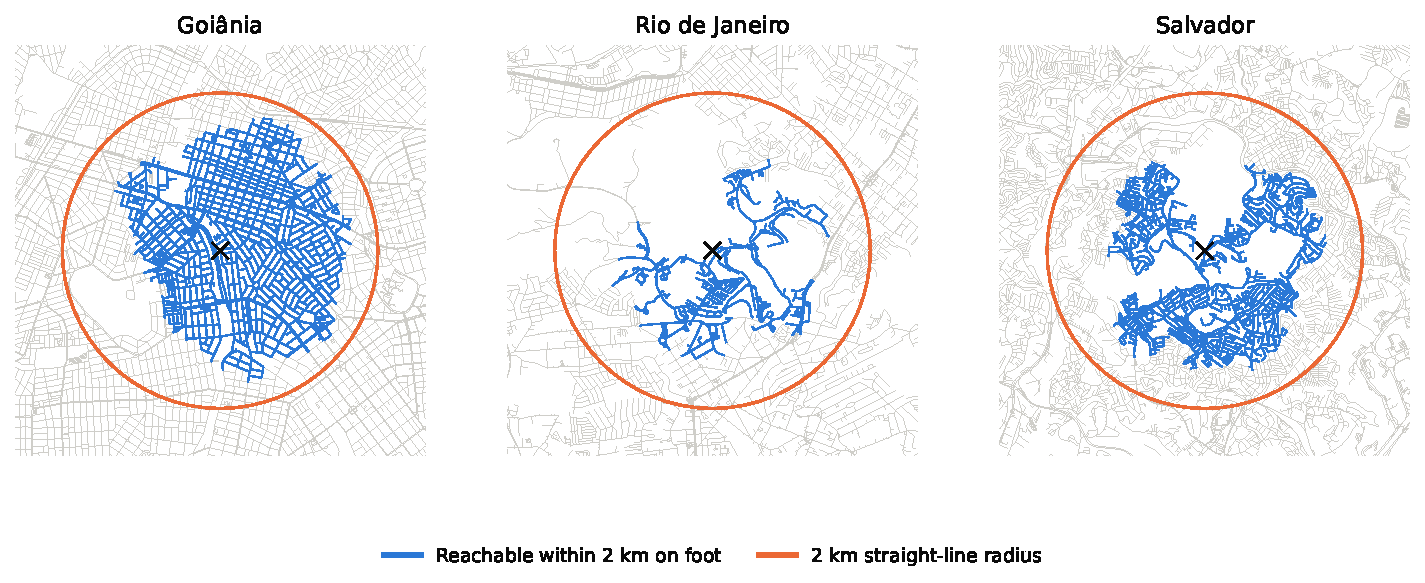
\includegraphics[width=\textwidth]{figures/fig1_vignettes.pdf}
\caption{Street segments reachable within 2~km on foot (blue) and the 2-km straight-line radius (orange) from
the node nearest the population-weighted centre of each city's urban tracts.}\label{fig:vignettes}
\end{figure}

Table~\ref{tab:gap} summarises the comparison for the main specification. Measured with network distance, the
spatial information theory index is higher in all \nCities{} municipalities (\sharePositive\%). The mean index
rises from \meanHeuc{} to \meanHnet{}, a mean relative increase of \meanPdH\%, larger than the $\approx$20\%
reported for US metropolitan areas by \citet{knaap2024segregated}. The relative gap ranges from \minPdH\% to
\maxPdH\%. Levels of racial segregation measured by $H$ are low in absolute terms, as expected for a
five-group index in cities where most residents are \emph{pardo} or white. The two measures are strongly
correlated across cities (Pearson \pearsonMain, Spearman \spearmanMain, Figure~\ref{fig:scatter}).

\begin{table}[htbp]
\centering\small
\caption{Spatial information theory index under Euclidean and network distance (2-km linear kernel,
\nCities{} municipalities). Gap $= H^{N} - H^{E}$; Gap (\%) $= 100\,(H^{N} - H^{E})/H^{E}$.}\label{tab:gap}
\begin{tabular}{lrrrrrrrr}
\toprule
 & count & mean & std & min & 25\% & 50\% & 75\% & max \\
\midrule
H, Euclidean & 91.000 & 0.022 & 0.017 & 0.001 & 0.009 & 0.017 & 0.032 & 0.072 \\
H, network & 91.000 & 0.028 & 0.020 & 0.002 & 0.011 & 0.022 & 0.040 & 0.079 \\
Gap & 91.000 & 0.005 & 0.005 & 0.000 & 0.002 & 0.004 & 0.007 & 0.026 \\
Gap (\%) & 91.000 & 29.835 & 18.968 & 0.751 & 16.294 & 25.209 & 39.522 & 108.987 \\
\bottomrule
\end{tabular}

\end{table}

\begin{figure}[htbp]
\centering
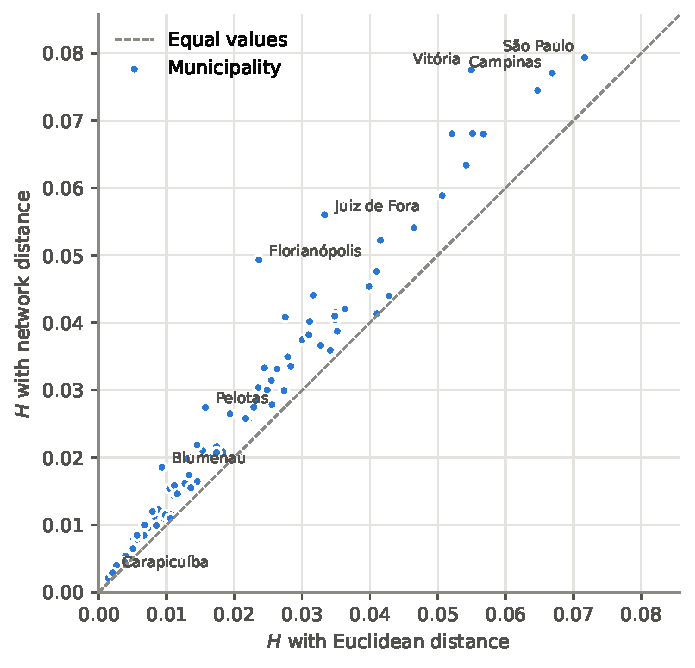
\includegraphics[width=0.6\textwidth]{figures/fig3_scatter.pdf}
\caption{$H$ under Euclidean and network distance. Points above the dashed line are cities where network
distance yields higher segregation. Labelled: the five largest relative gaps and the three highest network
values.}\label{fig:scatter}
\end{figure}

Despite the high correlation, the choice of metric changes the answer to the question most often asked of
segregation indices: which places are most segregated. Among the cities that rank in the top 15 under either
metric, \nRankChangeTop{} change position (Figure~\ref{fig:ranks}). The largest moves are cities built on
hills, islands and narrow valleys: Florian\'opolis rises from 38th to 13th, Juiz de Fora from 22nd to 10th and
Vit\'oria from 6th to 2nd. Bras\'ilia (11th to 17th) and Santos (13th to 20th) fall. The map in
Figure~\ref{fig:map} shows no simple regional pattern in the relative gap. Large gaps occur in the South (Florian\'opolis,
Blumenau, Pelotas), in Minas Gerais (Juiz de Fora), in peripheral municipalities of the S\~ao Paulo and Belo Horizonte
metropolitan areas (Carapicu\'iba, Diadema, Ribeir\~ao das Neves) and in Macei\'o.

\begin{figure}[htbp]
\centering
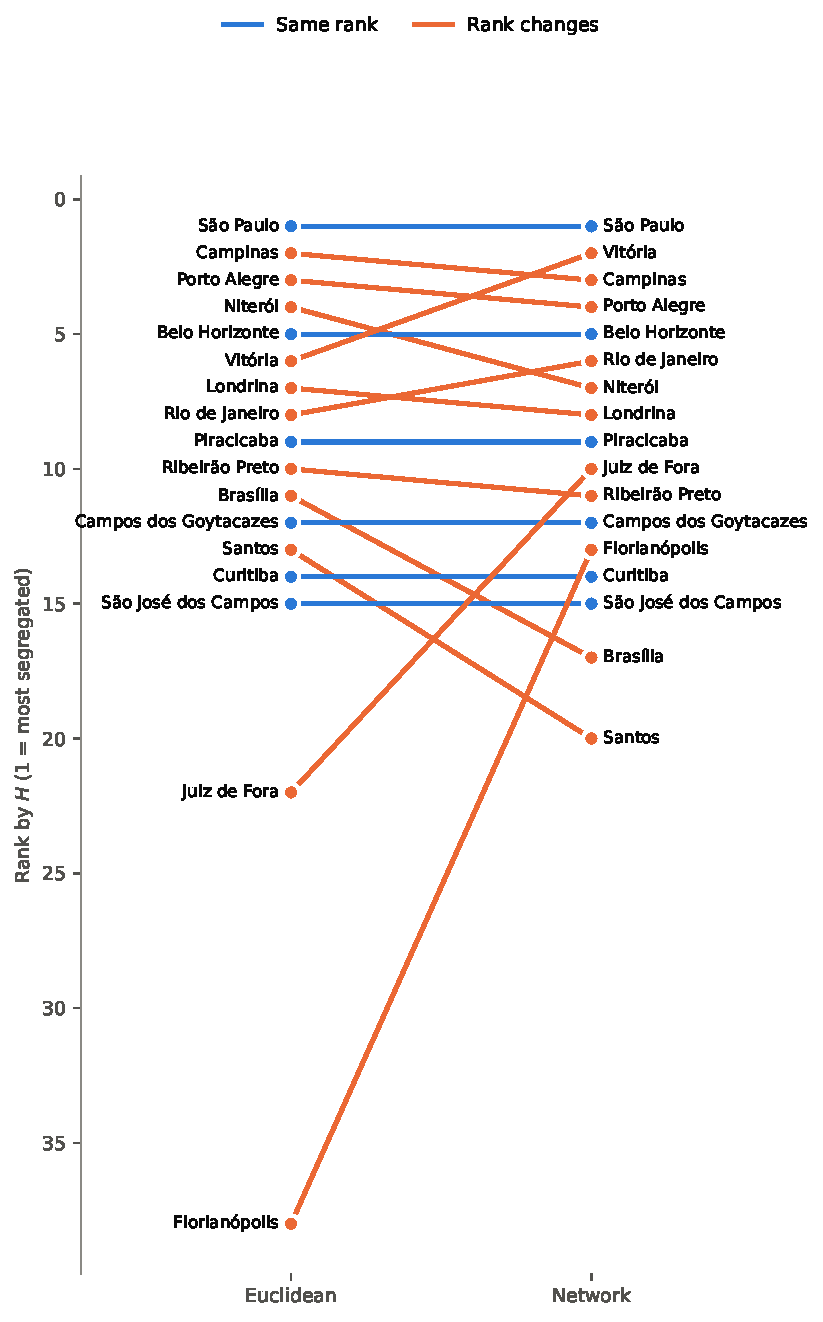
\includegraphics[width=0.62\textwidth]{figures/fig2_rank_slope.pdf}
\caption{Ranks of the most segregated municipalities (top 15 under either metric) with Euclidean and network
distance. Orange lines mark cities whose rank changes.}\label{fig:ranks}
\end{figure}

\begin{figure}[htbp]
\centering
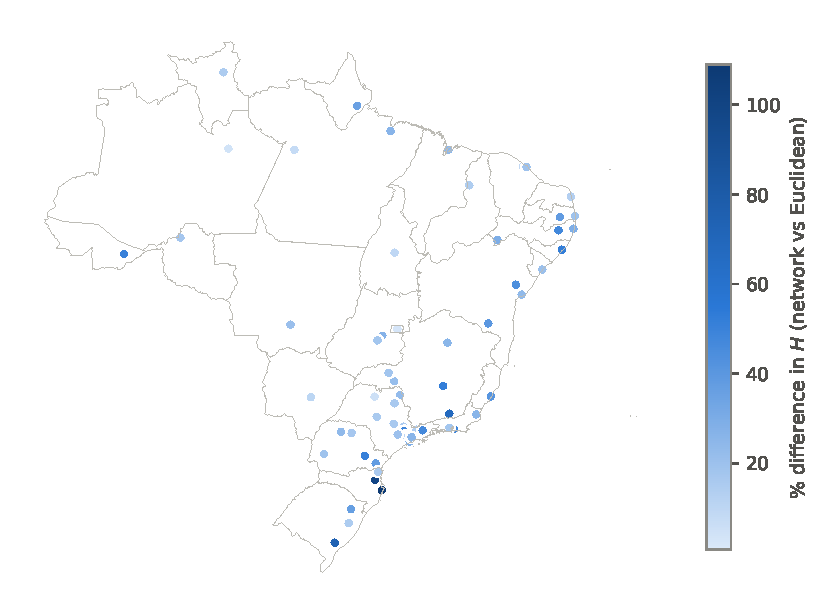
\includegraphics[width=0.72\textwidth]{figures/fig4_map_pdH.pdf}
\caption{Relative difference between network and Euclidean $H$ (\%) by municipality.}\label{fig:map}
\end{figure}

These results are robust to the kernel. With 1-km or 3-km bandwidths, an exponential kernel, or the
single-group dissimilarity and entropy indices for the \emph{preta}+\emph{parda} population, network-based
segregation remains higher in almost every city (Appendix Table~\ref{tab:robust}). The exception is the isolation
index, which changes little under either metric (its mean relative difference is below 2\% in every
specification).

\paragraph{Population-matched environments.} They are not robust, however, to holding the size of local
environments constant. Walking reaches far fewer people than a straight line: the mean 2-km network environment
contains \envPopRatio\% of the (kernel-weighted) population of the corresponding Euclidean environment (median
across cities), with a range of \ratioMin--\ratioMax\%. When each tract's Euclidean radius is shrunk until its
environment holds the same population as its network environment (median radius \medianPopmatchB~m), the gap
disappears. The mean relative difference becomes \meanPdHPopmatch\%, network $H$ exceeds the matched Euclidean $H$
in only \sharePositivePopmatch\% of cities, and the ranking under the two metrics becomes practically identical
(Spearman \spearmanPopmatch). The same holds for the single-group indices (Table~\ref{tab:robust}). In Brazilian
cities, therefore, the network--Euclidean gap is almost entirely a difference in the \emph{scale} of local
environments, as \citet{saporito2026reconsidering} argued for US cities, rather than evidence that the street
network separates groups beyond what a smaller neighbourhood would.

\subsection{Which network characteristics explain the gap?}

Figure~\ref{fig:clustermap} shows the correlation structure of the topology measures. As in
\citet{knaap2024segregated}, one cluster groups meshedness, gamma, streets per node and the share of 4-way
intersections (connectivity). A second groups circuity, dead-end share and self-loops (a dendritic, winding
fabric). A third groups size and density. Configurational fragmentation $F$ is nearly uncorrelated with all of
them. The relative gap belongs with the dendritic cluster: it rises with the dead-end share (Spearman
\rhoDeadEndPdH) and is essentially unrelated to $F$ (\rhoFragPdH).

\begin{figure}[htbp]
\centering
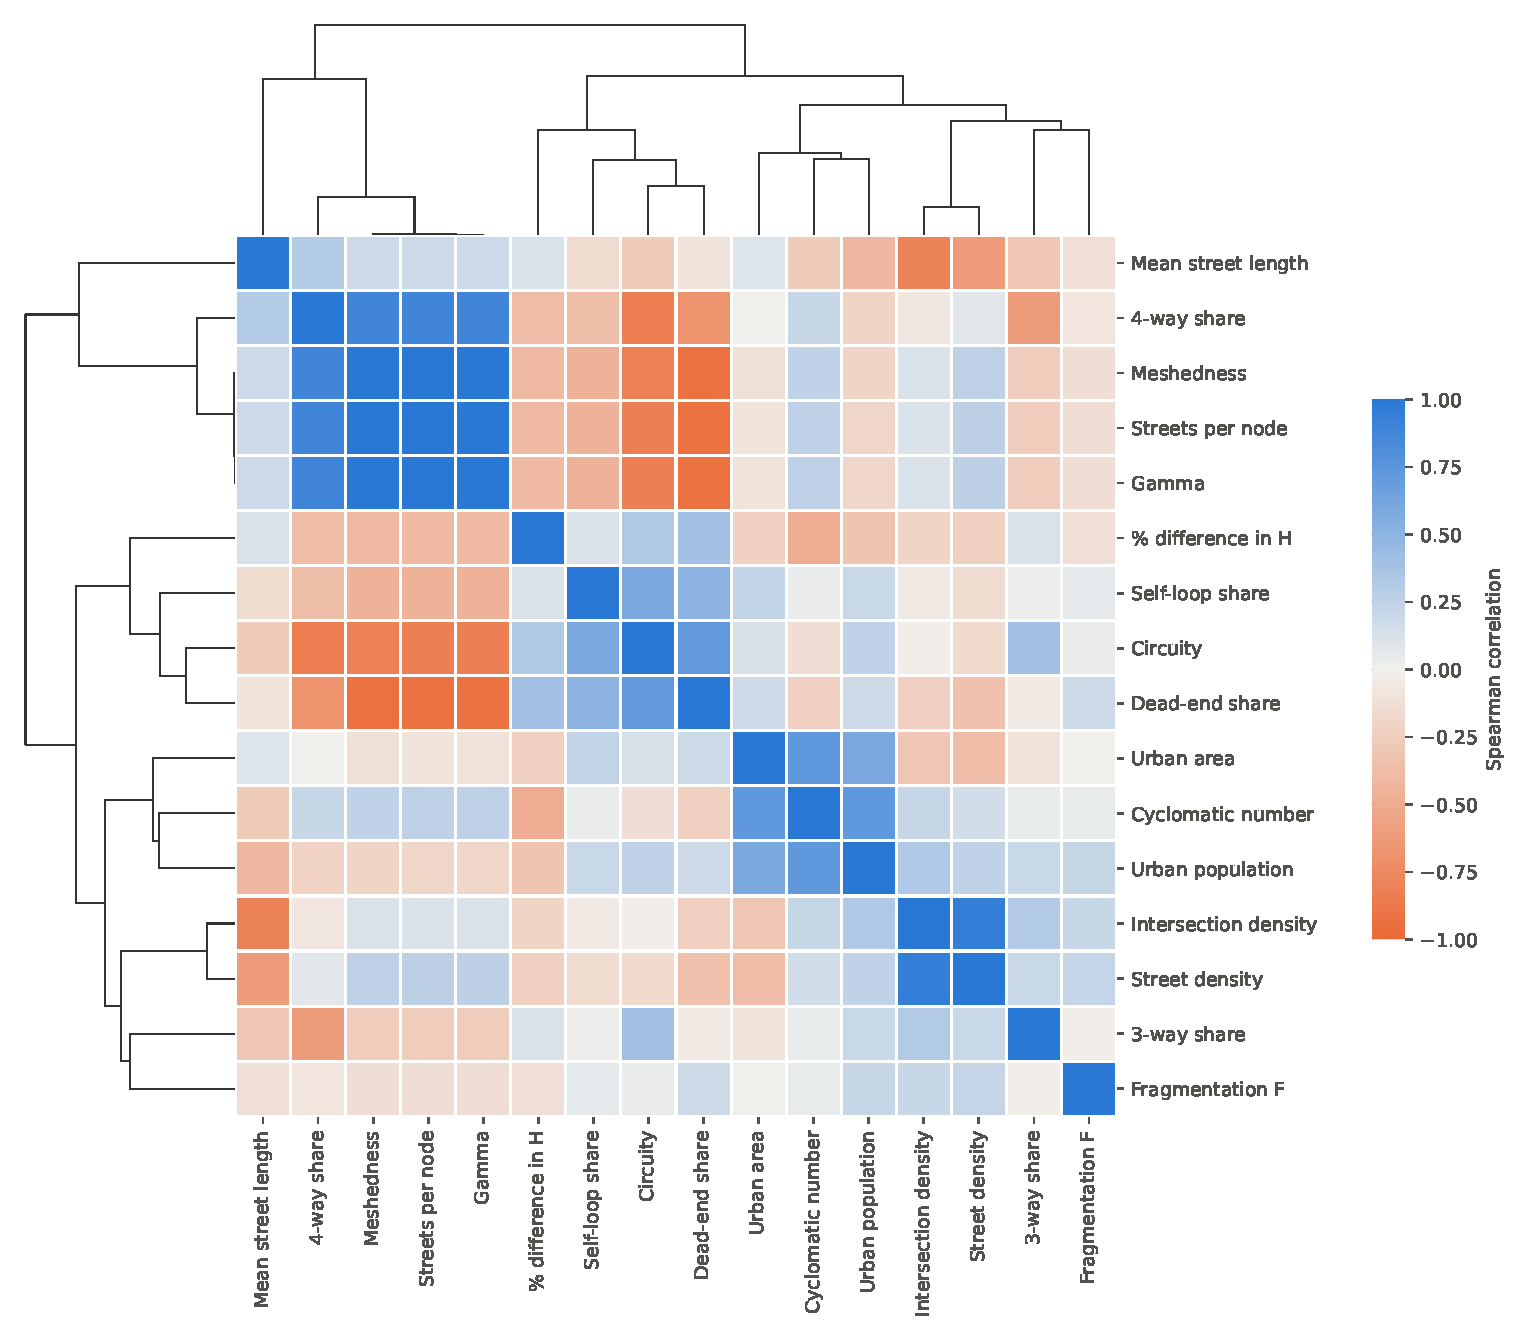
\includegraphics[width=0.8\textwidth]{figures/fig5_clustermap.pdf}
\caption{Spearman correlations among street-network topology measures, city size and the relative gap in
$H$, hierarchically clustered.}\label{fig:clustermap}
\end{figure}

Table~\ref{tab:models} reports the regressions. In all four models the dead-end share is positively associated
with both the absolute and the relative gap, and the level of Euclidean segregation is strongly associated with
the absolute gap (positively) and the relative gap (negatively). The negative association with the relative gap
means that low-segregation cities show larger relative differences, although the absolute differences there are
small. The cyclomatic number is negatively associated with the relative gap, consistent with more redundant
networks approximating unconstrained movement. Circuity, meshedness, intersection density and the
cyclomatic$\times$circuity interaction are not significant once the dead-end share is included. Meshedness and
the dead-end share are strongly collinear (variance inflation factors of 12.7 and 9.4), so their separate
coefficients should be read with caution. Adding fragmentation $F$ does not improve the fit: its coefficient is
small, negative and not significant, and the adjusted $R^2$ falls slightly. Figure~\ref{fig:frag} makes the
same point visually.

\begin{table}[htbp]
\centering\small
\caption{OLS models of the absolute ($\Delta H$) and relative (\%$\Delta H$) gap. K\&R: the specification of
\citet{knaap2024segregated}; +$F$: adding configurational fragmentation. Standardised (z) or logged regressors;
HC3 standard errors in parentheses. * $p<0.1$, ** $p<0.05$, *** $p<0.01$.}\label{tab:models}
\begin{tabular}{lrrrr}
\toprule
 & $\Delta H$ (K\&R) & $\Delta H$ (+$F$) & \%$\Delta H$ (K\&R) & \%$\Delta H$ (+$F$) \\
\midrule
Intersection density (log) & 0.0031 & 0.0030 & 14.34 & 13.66 \\
 & (0.0038) & (0.0039) & (9.46) & (9.39) \\
Circuity & 0.0001 & -0.0004 & 21.36 & 15.51 \\
 & (0.0072) & (0.0069) & (25.71) & (24.12) \\
Meshedness & 0.0015 & 0.0016 & -0.21 & -0.10 \\
 & (0.0018) & (0.0018) & (5.59) & (5.45) \\
Cyclomatic number (log) & -0.0017 & -0.0017 & -6.75** & -6.38* \\
 & (0.0011) & (0.0011) & (3.36) & (3.34) \\
Dead-end share & 0.0025** & 0.0026** & 9.14** & 9.68** \\
 & (0.0012) & (0.0012) & (4.46) & (4.30) \\
Population density (log) & -0.0027 & -0.0025 & -11.69* & -10.15 \\
 & (0.0022) & (0.0023) & (6.79) & (6.80) \\
$H$, Euclidean & 0.0030*** & 0.0030*** & -6.29*** & -6.40*** \\
 & (0.0005) & (0.0006) & (1.69) & (1.66) \\
Cyclomatic (log) $\times$ circuity & 0.0001 & 0.0002 & -2.23 & -1.58 \\
 & (0.0008) & (0.0007) & (2.87) & (2.68) \\
Fragmentation $F$ &  & -0.0002 &  & -2.16 \\
 &  & (0.0004) &  & (1.65) \\
Intercept & 0.0289** & 0.0277** & 121.95** & 109.01** \\
 & (0.0115) & (0.0127) & (47.90) & (50.25) \\
\midrule
$N$ & 91 & 91 & 91 & 91 \\
Adj. $R^2$ & 0.481 & 0.476 & 0.466 & 0.471 \\
\bottomrule
\end{tabular}

\end{table}

\begin{figure}[htbp]
\centering
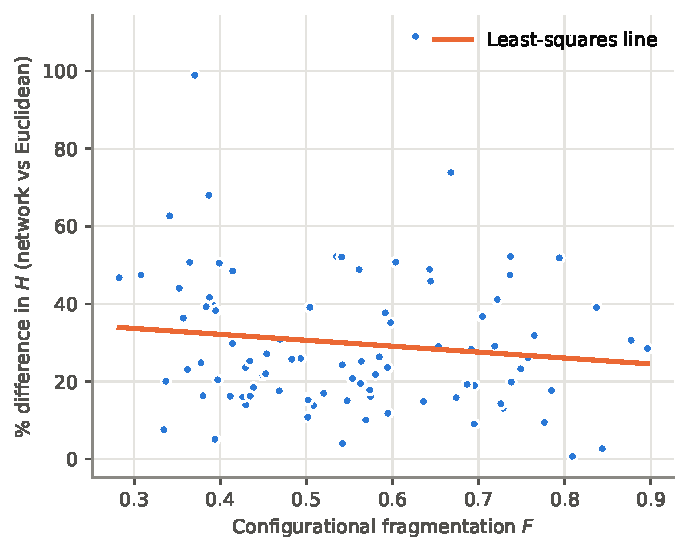
\includegraphics[width=0.55\textwidth]{figures/fig6_fragmentation.pdf}
\caption{Configurational fragmentation $F$ and the relative gap in $H$.}\label{fig:frag}
\end{figure}

The population-matched results suggest how topology matters. The share of the Euclidean population that is
reachable on foot is itself strongly associated with network form: it is lower where dead ends
(\rhoDeadEndRatio) and circuitous streets (\rhoCircuityRatio) are common and higher where the network is meshed
(\rhoMeshRatio), but it is unrelated to fragmentation (\rhoFragRatio). The gap is in turn larger where that
share is smaller (\rhoRatioPdH). Street topology thus shapes measured segregation mainly by setting the
effective scale of the neighbourhood.

\section{Discussion}\label{sec:discussion}

Our first result replicates, and amplifies, the central finding of \citet{knaap2024segregated}. When local
environments are defined by walking distance, racial segregation in large Brazilian cities is higher in every
case, by \meanPdH\% on average, and the ranking of the most segregated places changes. Cities built on hills,
islands and valleys (Florian\'opolis, Vit\'oria, Juiz de Fora) climb the ranking. Analysts who compare cities
with Euclidean spatial indices would therefore reach different conclusions about where segregation is most
intense. This is consistent with the Brazilian configurational literature, which describes Brazilian street
networks as unusually fragmented and labyrinthine \citep{medeiros2013urbis,holanda2002espaco}.

Our second result qualifies the first. Once the population of local environments is held constant, the gap
vanishes. Walking along the network does not reveal a different social composition next door. It reveals a
smaller neighbourhood, and smaller neighbourhoods are, as the multiscalar literature shows, more segregated
\citep{reardon2008geographic}. This supports the concern raised by \citet{saporito2026reconsidering} and changes
how the network--Euclidean gap should be read. It is not evidence that streets act as barriers that sort groups
within a given population radius. It is evidence that street networks set the \emph{effective scale} at which
residents experience their city: in dendritic, circuitous, cul-de-sac-rich fabrics, a 2-km walk reaches
as little as \ratioMin\% of the people a 2-km circle would. That is still a finding about urban design. Where the network
is poorly connected, the local environment of an average resident is smaller and therefore more homogeneous,
which matters for everyday exposure to other groups \citep{netto2015segregated}. But it calls for a different
framing, and for population-based (or population-matched) comparisons whenever network and Euclidean indices are
contrasted.

Third, we find no support for configurational fragmentation, as we operationalise it, as a predictor of the gap.
Neither the gap nor the share of reachable population is associated with $F$. What matters is the local
texture of the network: dead ends, circuity and meshedness. These are exactly the features that gated
condominiums and closed \emph{loteamentos} produce \citep{coy2006gated}. One interpretation is that
local-environment indices at a 2-km scale are sensitive to local permeability and blind to city-wide
articulation, the property that synergy captures. Another is that our metric analogue does not capture what
space-syntax synergy measures on axial maps. Testing CHASM-type segment-based measures \citep{saboya2025chasm},
which build the street grid into exposure itself, is a natural next step.

\paragraph{Limitations.} First, OpenStreetMap coverage of informal settlements is uneven: stairways and alleys
in favelas are often missing, which lengthens network paths and may inflate the gap there, so our estimates for
hillside cities are best read as upper bounds. Second, tracts are represented by a single interior point, and
\nSnapFar{} of the \nTractsUrban{} tracts lie more than 500~m from the nearest network node. Third, we consider the
walking network only; public transport would lengthen reach and probably reduce the gap
\citep{pereira2021r5r,bittencourt2021cumulative}. Fourth, the units are municipalities, not functional urban
areas, and results are subject to the modifiable areal unit problem. Finally, following the design of this paper,
we do not test whether the gaps are larger than would be expected by chance. The random-labelling framework of
\citet{rey2021comparative} and \citet{knaap2024segregated} can be applied directly to our cached weights.

\section{Conclusion}\label{sec:conclusion}

Measured with walking distance, racial segregation in the \nCities{} largest Brazilian municipalities is
uniformly higher than when measured as the crow flies, and rankings of the most segregated cities change. But
the difference disappears once local environments are matched in population. The street network shapes measured
segregation mainly by shrinking the neighbourhood rather than by separating groups within it. Dead ends and
circuity, not city-wide configurational fragmentation, are associated with that shrinkage. For measurement, this
means that network and Euclidean indices should be compared at equal population scale. For planning, it points to
the permeability of the local street fabric, the connectivity of peripheral \emph{loteamentos} and gated enclaves,
as the lever through which urban design conditions everyday exposure between racial groups. Future work should
add inferential tests of the gap, multiscalar profiles, and public-transport networks.


\section*{Code and data availability}
All code is in a self-contained companion repository (URL withheld during review) and reproduces every number,
table and figure from public inputs. Census tract counts and geometries are from IBGE (2022 Census). Street
networks are \copyright{} OpenStreetMap contributors (ODbL); download dates are recorded per city. Unit tests
verify, among other things, that our local-environment computation reproduces the PySAL \texttt{segregation}
\texttt{w=} path to machine precision.

\bibliography{references}

\appendix
\section{Robustness}\label{app:robust}

\begin{table}[H]
\centering\footnotesize
\caption{Network versus Euclidean indices under alternative specifications (\nCities{} municipalities). ``Mean
gap (\%)'' is the mean of $100\,(I^{N} - I^{E})/I^{E}$; ``Share gap $>$ 0'' is the share of cities in which the
network index is higher. PP: \emph{preta}+\emph{parda}. Population-matched: Euclidean radii shrunk tract by tract
to match the population of 2-km network environments.}\label{tab:robust}
\begin{tabular}{llrrrrr}
\toprule
Specification & Index & Mean gap & Mean gap (\%) & Share gap > 0 & Pearson & Spearman \\
\midrule
2 km, linear & H (five groups) & 0.005 & 29.835 & 1.000 & 0.980 & 0.984 \\
2 km, linear & Dissimilarity (PP) & 0.018 & 12.663 & 0.978 & 0.985 & 0.982 \\
2 km, linear & Isolation (PP) & 0.003 & 0.665 & 0.692 & 0.999 & 0.999 \\
2 km, linear & Entropy (PP) & 0.007 & 28.761 & 1.000 & 0.982 & 0.986 \\
1 km, linear & H (five groups) & 0.007 & 28.578 & 0.989 & 0.984 & 0.988 \\
1 km, linear & Dissimilarity (PP) & 0.017 & 10.965 & 0.978 & 0.989 & 0.984 \\
1 km, linear & Isolation (PP) & 0.004 & 1.152 & 0.802 & 0.999 & 0.999 \\
1 km, linear & Entropy (PP) & 0.008 & 24.604 & 0.978 & 0.987 & 0.988 \\
3 km, linear & H (five groups) & 0.005 & 36.901 & 1.000 & 0.983 & 0.985 \\
3 km, linear & Dissimilarity (PP) & 0.018 & 16.117 & 0.978 & 0.983 & 0.982 \\
3 km, linear & Isolation (PP) & 0.001 & 0.336 & 0.604 & 0.999 & 0.999 \\
3 km, linear & Entropy (PP) & 0.006 & 37.179 & 1.000 & 0.984 & 0.986 \\
2 km, exponential & H (five groups) & 0.005 & 28.481 & 0.989 & 0.983 & 0.986 \\
2 km, exponential & Dissimilarity (PP) & 0.017 & 11.861 & 0.967 & 0.987 & 0.984 \\
2 km, exponential & Isolation (PP) & 0.003 & 0.683 & 0.714 & 0.999 & 0.999 \\
2 km, exponential & Entropy (PP) & 0.006 & 26.950 & 0.989 & 0.985 & 0.988 \\
Population-matched & H (five groups) & -0.000 & -1.577 & 0.209 & 0.999 & 0.999 \\
Population-matched & Dissimilarity (PP) & -0.001 & -0.652 & 0.319 & 0.999 & 0.999 \\
Population-matched & Isolation (PP) & -0.001 & -0.265 & 0.286 & 1.000 & 1.000 \\
Population-matched & Entropy (PP) & -0.000 & -1.382 & 0.253 & 0.999 & 0.999 \\
\bottomrule
\end{tabular}

\end{table}

\begin{table}[H]
\centering\footnotesize
\caption{Street-network topology across the \nCities{} municipalities.}\label{tab:topodesc}
\resizebox{\textwidth}{!}{\begin{tabular}{lrrrrrrrr}
\toprule
 & count & mean & std & min & 25\% & 50\% & 75\% & max \\
\midrule
Intersection density (per km2) & 91.000 & 96.167 & 42.444 & 30.803 & 66.511 & 93.617 & 112.886 & 286.045 \\
Street density (km/km2) & 91.000 & 13.374 & 3.844 & 5.860 & 10.458 & 13.507 & 15.310 & 24.892 \\
Mean street length (m) & 91.000 & 85.027 & 12.286 & 50.293 & 76.284 & 84.081 & 93.440 & 110.996 \\
Streets per node & 91.000 & 2.878 & 0.164 & 2.334 & 2.773 & 2.880 & 2.995 & 3.254 \\
Circuity & 91.000 & 1.045 & 0.016 & 1.018 & 1.033 & 1.043 & 1.054 & 1.112 \\
Dead-end share & 91.000 & 0.149 & 0.052 & 0.054 & 0.116 & 0.145 & 0.178 & 0.360 \\
3-way share & 91.000 & 0.636 & 0.055 & 0.468 & 0.593 & 0.645 & 0.679 & 0.732 \\
4-way share & 91.000 & 0.194 & 0.074 & 0.062 & 0.143 & 0.175 & 0.229 & 0.404 \\
Cyclomatic number & 91.000 & 9371.341 & 11411.163 & 1834.000 & 4142.000 & 6243.000 & 9468.000 & 86122.000 \\
Meshedness & 91.000 & 0.221 & 0.041 & 0.084 & 0.194 & 0.221 & 0.250 & 0.314 \\
Gamma & 91.000 & 0.480 & 0.027 & 0.389 & 0.462 & 0.480 & 0.499 & 0.542 \\
F & 91.000 & 0.552 & 0.152 & 0.283 & 0.420 & 0.542 & 0.680 & 0.896 \\
\bottomrule
\end{tabular}
}
\end{table}

Configurational fragmentation is estimated from random samples of 500 targets and 2,000 origins per city. Doubling
both samples changes $F$ by less than 0.02 in Porto Alegre, Curitiba and Salvador.

\section{Cross-check against the native PySAL network route}\label{app:pandana}

Using the \texttt{pandana} library, the PySAL \texttt{segregation} package can also build network-based
local environments itself \citep{cortes2026segregation}. That route aggregates population at the network node nearest to
each tract and ignores the distance between the tract point and the node. For Porto Alegre, Curitiba and Salvador
it yields network $H$ within 0.001 of our estimates (Table~\ref{tab:pandana}).

\begin{table}[H]
\centering\small
\caption{Network $H$ from our tract-to-tract weights and from \texttt{segregation}'s native \texttt{pandana}
route.}\label{tab:pandana}
\begin{tabular}{lrrr}
\toprule
City & H, Euclidean & H, network (ours) & H, network (pandana) \\
\midrule
Porto Alegre & 0.0647 & 0.0745 & 0.0736 \\
Curitiba & 0.0410 & 0.0476 & 0.0472 \\
Salvador & 0.0310 & 0.0382 & 0.0382 \\
\bottomrule
\end{tabular}

\end{table}

\section{City-level results}\label{app:cities}

{\footnotesize
\begin{longtable}{lrrrr}
\toprule
City & H, Euclidean & H, network & Gap (\%) & F \\
\midrule
\endfirsthead
\toprule
City & H, Euclidean & H, network & Gap (\%) & F \\
\midrule
\endhead
\midrule
\multicolumn{5}{r}{Continued on next page} \\
\midrule
\endfoot
\bottomrule
\endlastfoot
Florianópolis & 0.024 & 0.049 & 108.987 & 0.627 \\
Blumenau & 0.009 & 0.019 & 98.939 & 0.370 \\
Pelotas & 0.016 & 0.027 & 73.877 & 0.668 \\
Juiz de Fora & 0.033 & 0.056 & 67.987 & 0.387 \\
Carapicuíba & 0.002 & 0.003 & 62.676 & 0.341 \\
Ribeirão das Neves & 0.001 & 0.002 & 52.246 & 0.535 \\
Maceió & 0.013 & 0.020 & 52.226 & 0.737 \\
Diadema & 0.005 & 0.008 & 52.102 & 0.541 \\
Serra & 0.008 & 0.012 & 51.846 & 0.794 \\
Ananindeua & 0.003 & 0.004 & 50.797 & 0.604 \\
Ponta Grossa & 0.014 & 0.022 & 50.716 & 0.365 \\
Rio Branco & 0.006 & 0.008 & 50.512 & 0.399 \\
Itaquaquecetuba & 0.002 & 0.003 & 48.926 & 0.643 \\
São Gonçalo & 0.006 & 0.008 & 48.858 & 0.561 \\
Jundiaí & 0.028 & 0.041 & 48.494 & 0.414 \\
Caruaru & 0.003 & 0.004 & 47.485 & 0.308 \\
Jaboatão dos Guararapes & 0.007 & 0.010 & 47.451 & 0.737 \\
Taubaté & 0.010 & 0.015 & 46.754 & 0.283 \\
Paulista & 0.003 & 0.004 & 45.872 & 0.644 \\
Feira de Santana & 0.006 & 0.009 & 44.053 & 0.352 \\
Mauá & 0.011 & 0.016 & 41.736 & 0.388 \\
Vitória & 0.055 & 0.078 & 41.150 & 0.722 \\
Vitória da Conquista & 0.009 & 0.012 & 39.770 & 0.391 \\
São Bernardo do Campo & 0.032 & 0.044 & 39.275 & 0.384 \\
Canoas & 0.012 & 0.016 & 39.116 & 0.504 \\
Belford Roxo & 0.002 & 0.003 & 39.074 & 0.837 \\
Campina Grande & 0.006 & 0.008 & 38.264 & 0.395 \\
São José dos Pinhais & 0.015 & 0.021 & 37.706 & 0.592 \\
Praia Grande & 0.019 & 0.026 & 36.760 & 0.704 \\
Caxias do Sul & 0.024 & 0.033 & 36.372 & 0.357 \\
Macapá & 0.004 & 0.005 & 35.155 & 0.598 \\
Olinda & 0.007 & 0.010 & 31.846 & 0.765 \\
Cariacica & 0.013 & 0.017 & 30.853 & 0.469 \\
Rio de Janeiro & 0.052 & 0.068 & 30.621 & 0.877 \\
Petrolina & 0.008 & 0.011 & 29.791 & 0.414 \\
Recife & 0.031 & 0.040 & 29.134 & 0.719 \\
São Vicente & 0.024 & 0.030 & 29.057 & 0.653 \\
Duque de Caxias & 0.005 & 0.006 & 28.477 & 0.896 \\
Nova Iguaçu & 0.011 & 0.014 & 28.329 & 0.692 \\
Anápolis & 0.013 & 0.016 & 27.118 & 0.454 \\
Belém & 0.012 & 0.015 & 26.333 & 0.585 \\
Contagem & 0.007 & 0.008 & 26.041 & 0.758 \\
Suzano & 0.026 & 0.033 & 25.976 & 0.494 \\
Campos dos Goytacazes & 0.042 & 0.052 & 25.748 & 0.483 \\
Montes Claros & 0.012 & 0.015 & 25.303 & 0.434 \\
Barueri & 0.028 & 0.035 & 25.209 & 0.564 \\
Mogi das Cruzes & 0.030 & 0.037 & 24.837 & 0.378 \\
São Luís & 0.017 & 0.022 & 24.293 & 0.542 \\
Maringá & 0.025 & 0.031 & 23.598 & 0.429 \\
Belo Horizonte & 0.055 & 0.068 & 23.561 & 0.594 \\
Salvador & 0.031 & 0.038 & 23.264 & 0.749 \\
Franca & 0.017 & 0.021 & 23.131 & 0.362 \\
Betim & 0.007 & 0.008 & 22.015 & 0.453 \\
Vila Velha & 0.031 & 0.038 & 21.852 & 0.580 \\
Uberaba & 0.023 & 0.028 & 21.662 & 0.449 \\
Cuiabá & 0.025 & 0.030 & 20.817 & 0.553 \\
Aracaju & 0.017 & 0.020 & 20.423 & 0.397 \\
Sorocaba & 0.023 & 0.027 & 20.049 & 0.337 \\
Niterói & 0.057 & 0.068 & 19.870 & 0.738 \\
Fortaleza & 0.017 & 0.021 & 19.495 & 0.563 \\
João Pessoa & 0.022 & 0.026 & 19.249 & 0.687 \\
Cascavel & 0.035 & 0.042 & 19.029 & 0.695 \\
Uberlândia & 0.028 & 0.034 & 18.436 & 0.439 \\
Goiânia & 0.035 & 0.041 & 17.824 & 0.574 \\
São João de Meriti & 0.004 & 0.005 & 17.682 & 0.785 \\
Porto Velho & 0.010 & 0.012 & 17.604 & 0.469 \\
Londrina & 0.054 & 0.063 & 16.990 & 0.520 \\
Ribeirão Preto & 0.046 & 0.054 & 16.330 & 0.380 \\
Curitiba & 0.041 & 0.048 & 16.257 & 0.435 \\
Piracicaba & 0.051 & 0.059 & 16.229 & 0.412 \\
Joinville & 0.022 & 0.026 & 16.098 & 0.575 \\
Santo André & 0.035 & 0.040 & 16.029 & 0.426 \\
Aparecida de Goiânia & 0.009 & 0.010 & 15.857 & 0.674 \\
Bauru & 0.036 & 0.042 & 15.675 & 0.502 \\
Campinas & 0.067 & 0.077 & 15.247 & 0.502 \\
Porto Alegre & 0.065 & 0.074 & 15.031 & 0.547 \\
Boa Vista & 0.010 & 0.011 & 14.911 & 0.636 \\
Teresina & 0.014 & 0.016 & 14.292 & 0.726 \\
Osasco & 0.018 & 0.021 & 13.971 & 0.430 \\
São José dos Campos & 0.040 & 0.045 & 13.827 & 0.509 \\
Natal & 0.015 & 0.016 & 13.090 & 0.729 \\
Guarulhos & 0.033 & 0.037 & 11.837 & 0.595 \\
São Paulo & 0.072 & 0.079 & 10.791 & 0.502 \\
Campo Grande & 0.035 & 0.039 & 10.096 & 0.569 \\
Palmas & 0.027 & 0.030 & 9.485 & 0.776 \\
Caucaia & 0.026 & 0.028 & 9.060 & 0.695 \\
Santarém & 0.011 & 0.012 & 7.579 & 0.335 \\
São José do Rio Preto & 0.034 & 0.036 & 5.132 & 0.394 \\
Manaus & 0.011 & 0.011 & 4.019 & 0.542 \\
Brasília & 0.043 & 0.044 & 2.716 & 0.844 \\
Santos & 0.041 & 0.041 & 0.751 & 0.809 \\
\end{longtable}

}

\end{document}
